\begin{quotation}[TODO Sophie Meiss]
De même en trigonométrie, ton cours reste à illustrer pour lui donner du 
sens (l'enroulement de la droite réelle sur le cercle trigo peut se 
faire sous geogébra \ldots); dans le paragraphe 3 tu indiques la notation 
d'angle orienté de vecteurs qui n'est pas au programme en seconde. Sans 
définir le radian, il est préférable de rester sur le point associé à x 
(abscisse sur la droite réelle); il faut préciser également l'importance 
du sens trigonométrique.
\end{quotation}

\section{Cercle trigonométrique}

\begin{multicols}{2}
\begin{definition}
  On appelle \emph{cercle trigonométrique} le cercle de centre $O$, de rayon 1.
\end{definition}

\begin{center}
    \begin{tikzpicture}[scale=2]
      \draw (0,0) circle (1);
      \draw (-1.1,0) -- (1.1,0);
      \draw (0,-1.1) -- (0,1.1);
      \draw (1,0) node[below right]{$I$};
      \draw (0,1) node[above right]{$J$};
      \draw (0,0) node[below left]{$O$};
    \end{tikzpicture}
\end{center}
\end{multicols}

\section{Enroulement de la droite des réels}

\begin{multicols}{2}
On considère le cercle trigonométrique $\mathcal C$, et la droite $\mathcal D$ d'équation $x=1$. En « enroulant » cette droite autour du cercle $\mathcal C$, on obtient une correspondance entre un point $N$ de la droite et un unique point $M$ du cercle.

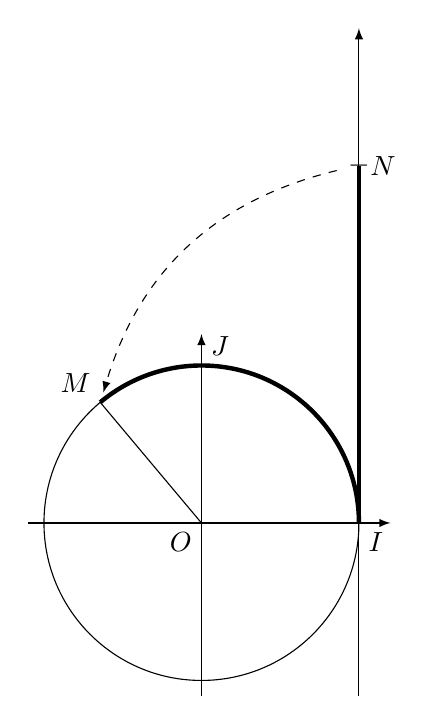
\begin{tikzpicture}[scale=2]
  \draw (0,0) circle (1);
  \draw[-latex] (-1.1,0) -- (1.2,0);
  \draw[-latex] (0,-1.1) -- (0,1.2);
  \draw (1,0) node[below right]{$I$};
  \draw (0,1) node[above right]{$J$};
  \draw (0,0) node[below left]{$O$};
  \draw[-latex] (1, -1.1) -- (1,pi);

  \draw[ultra thick] (1,0) -- (1, {130/180*pi}) node(N){$-$} node[right]{$N$};

  \draw (0,0) -- ({cos(130)}, {sin(130)}) node(M){} node[above left]{$M$};
  \draw[ultra thick] (1,0) arc (0:130:1);
  \draw[dashed,-latex] (N) to[bend right] (M);
\end{tikzpicture}
\end{multicols}

\section{Sinus et cosinus}

\begin{multicols}{2}
  \begin{propriete}
    Soit $M$ un point du cercle trigonométrique, la mesure de l'angle $(\vecteur{OI};\vecteur{OM})$ étant noté $t$. Ses coordonnées sont alors $\coord{\cos t}{\sin t}$.
  \end{propriete}
  \begin{demo}
    \emph{TODO : Triangle rectangle dans le cercle trigonométrique}.
  \end{demo}

  \columnbreak

  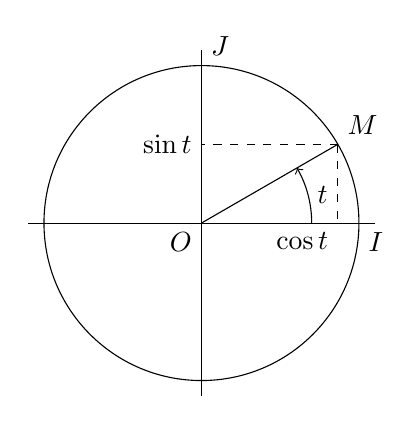
\begin{tikzpicture}[scale=2]
    \draw (0,0) circle (1);
    \draw (-1.1,0) -- (1.1,0);
    \draw (0,-1.1) -- (0,1.1);
    \draw (1,0) node[below right]{$I$};
    \draw (0,1) node[above right]{$J$};
    \draw (0,0) node[below left]{$O$};

    \draw (0,0) -- ({cos(30)}, {sin(30)}) node[above right]{$M$};
    \draw[->] (0.7,0) arc (0:30:0.7) node at ({0.7*cos(15)},{0.7*sin(15)})[right]{$t$};
    \draw[dashed] ({cos(30)}, {sin(30)}) -- ({cos(30)}, 0) node[below left]{$\cos t$};
    \draw[dashed] ({cos(30)}, {sin(30)}) -- (0, {sin(30)}) node[left]{$\sin t$};
  \end{tikzpicture}
\end{multicols}

\begin{propriete}Soit $t$ un réel.
  \begin{enumerate}[(i)]
    \item $\sin^2x+\cos^2x=1$
    \item $-1\leq\sin x\leq1$ et $-1\leq\cos x\leq1$
    \item $\sin-x=-\sin x$ et $\cos-x=\cos x$
  \end{enumerate}
\end{propriete}

\begin{propriete}[Valeurs particulières]

  \[
    \begin{array}{c||c|c|c|c|c}
      \alpha & 0\degree & 30\degree & 45\degree & 60\degree & 90\degree \\
      \hline
      \cos\alpha & 1 & \frac{\sqrt{3}}{2} & \frac{\sqrt{2}}{2} & \frac{1}{2} & 0 \\
      \hline
      \sin\alpha & 0 & \frac{1}{2} & \frac{\sqrt{2}}{2} & \frac{\sqrt{3}}{2} & 1 \\
    \end{array}
  \]
\end{propriete}
\begin{demo}
  Calculer la valeur et les sinus et cosinus des angles $\alpha$, $\beta$ et $\gamma$ suivants, dans les triangles suivants, dont l'un est rectangle isocèle, et l'autre est la moitié d'un triangle équilatéral.

  \vspace{1em}

  \hspace*{\stretch{1}}
  \begin{tikzpicture}[scale=3]
    \draw[thick] (0,1) -- (0,0) node[midway,left]{1} -- (1,0) node[midway,below]{1} -- cycle;
    \draw (0,0.1) -- (0.1,0.1) -- (0.1,0);
    \draw (0.7,0) arc (180:135:0.3);
    \draw ($(1,0) + (142.5:0.3)$) node[left]{$\alpha$};
  \end{tikzpicture}
  \hspace*{\stretch{1}}
  \begin{tikzpicture}[scale=3]
    \draw[thick] (0,0) -- (30:1) node[midway,above left]{1} -- ++(0,-0.5) node[midway,right]{$^1/_2$} -- cycle;
    \draw[dashed] (0,0) -- (-30:1) -- ++(0,0.5);
    \draw ({sqrt(3)/2},0.1) -- ++(-0.1,0) -- ++(0,-0.1);

    \draw (0.3,0) arc (0:30:0.3);
    \draw (15:0.3) node[right]{$\beta$};

    \draw ({sqrt(3)/2},0.3) arc (-90:-133:0.3);
    \draw ($(30:1) + (-110:0.3)$) node[]{$\gamma$};
  \end{tikzpicture}
  \hspace*{\stretch{1}}
\end{demo}

\section{Équations}

TODO Déterminer $cos x$ connaissant $\sin x$ et un intervalle auquel
appartient $x$.
